\documentclass{article}
\usepackage{fullpage}
\usepackage[czech]{babel}
\usepackage{amsfonts}
\usepackage{graphicx}
\usepackage{caption}
\graphicspath{{images/}}

\title{\vspace{-2cm}kmen Strunatci\vspace{-1.7cm}}
\date{}
\author{}

\begin{document}

\maketitle

aaaaa věci minulý úterý 14. 2.
\begin{itemize}
  \item obsahuje nadtřídy Bezčelistnatci a Čelistnatci
\end{itemize}

\section{nadtřída Bezčelistnatci}

\subsection{třída Sliznatky}
\begin{itemize}
  \item nejprimitivnější obratlovci, podobní rybám, až 1 m velcí
  \item mají zachovanou chordu, která je místy prostoupena základy obratlů
  \item obývají dna chladnějších mělkých moří v oblasti mírného pásu, jsou slepé
\end{itemize}

\subsection{třída Mihule}
\begin{itemize}
  \item až 1 m dlouhé hadovité tělo, v zadní polovině těla mají souvislý ploutevní lem
  \item zachovaná chorda, chrupavčitá, málo vyvinutá kostra, mají vyvinuté oči
  \item larva minoha, žije 2 až 5 let, připomíná kopinatce, dlouho si mysleli, že je samostatný druh
  \item mihule mořská, říční, potoční (u nás, teď málo častá)
\end{itemize}

\section{nadtřída Čelistnatci}

\subsection{třída Paryby}
\begin{itemize}
  \item starý druh, již od ordoviku, a to nezměněni (evolučně tedy poměrně dokonalí)
  \item končetiny ve tvaru ploutví -- párové prsní, párové břišní, ne-- i párová hřbetní, řitní, nesouměrná (u žraloků heterocerkní -- nestejně rozdvojená) ocasní
  \item mají žaberní štěrbiny a neumí polykat, nedýchají ,,aktivně" a musí tedy (třeba i ve spánku) plavat, aby se neudusili
  \item třetí víčko -- mžurka, chrání oči
  \item zahrnuje Chiméry (nějaký sea monsters z hlubin) a Příčnoústé (žraloci, rejnoci)
\end{itemize}

\subsubsection{podtřída Chiméry}
\begin{itemize}
  \item hlubokomořské, např. chiméra podivná
\end{itemize}

\subsubsection{podtřída Příčnoústí}
\begin{itemize}
  \item tvar těla torpédovitý, dorsoventrálně (zádo-břichově) zploštělý
  \item dlouhý rypec (rypák), ústa na spodní straně hlavy
  \item plakoidní šupiny -- podobné zubům (tvořené dentinem (naše zuby) a kryta emailem), orientované -- živočich hydrodynamičtější, ochrana před parasity
  \item chorda dorsalis zatlačena/potlačena obratly
  \item 5 žaberních štěrbin
  \item dominantní smysl čich a v rypci mají Lorenziho ampule -- velké množství volných nervových zakončení, které vnímá elektrické impulsy -- vnímá např. el. impulsy srdcí kořisti
  \item trvale se vyměňující zuby, zahnuté dovnitř
  \item lebka je široká, s pouzdry smyslových orgánů, dolní čelist uchycena na delším segmentu než např. naše -- mnohem silnější stisk
  \item soustava rozmnožovací a močová u samců propojeny, vejcorodí i nepravě živorodí (ve vejci, ale vejce v matce)
  \item zřídka i sladkovodní žraloci, žraloci buď predátoři, filtrátoři, nebo plují při dnu a loví korýše ap.
  \item patří sem žraloci -- žralok obrovský, žralok bílý, máčka skvrnitá; taky rejnoci -- rejnok ostnatý, parejnok elektrický, manta obrovská
\end{itemize}

\section{nadtřída Ryby}
\begin{itemize}
  \item mají kosti, mají žábra, gonochoristé, vnější rozmnožování
\end{itemize}

\subsection{třída Dvojdyšní}%dvojdyšní a lalokoploutví doopravdy řád, společně v třídě Nozdratí AAAAAAAA
\begin{itemize}
  \item NESTÍHÁM AAAAAAA
\end{itemize}

\subsection{třída Lalokoploutví}
\begin{itemize}
  \item dnes již téměř vyhynulá skupina, mají svalnaté ploutve, které používají jako \uv{nohy}, pohybují se po dně, pravděpodobně předchůdci suchozemských živočichů (včetně nás)
  \item např. latimérie podivná
\end{itemize}

\subsection{třída Paprskoploutví}
\begin{itemize}
  \item ryby podle \uv{tradičního} chápání
  \item nejpočetnější skupina obratlovců (moře je větší než souš)
  \item vodní obratlovci, prvotně vznikli ve sladkovodním prostředí
  \item převažují kosti nad chrupavkami (až na chrupavčité)
  \item ve škáře šupiny -- derivát pokožky (rozdílné od paryb)
  \item žaberní přepážky redukovány, žaberní dutina kryta skřelemi -- můžou aktivně dýchat, tj. se neutopí, když se zastaví
  \item tělo má hydrodynamciký tvar (proč asi)
  \item kůže obsahuje slizotvorné žlázy, pigmenty a šupiny, ty jsou:
\end{itemize}

\hspace{-0.03185\textwidth}\begin{minipage}{0.275\textwidth}\raggedleft
  \begin{itemize}
    \item[]
    \begin{itemize}
      \item ganoidní -- jeseter
      \item cykloidní -- kapr
      \item ktenoidní -- okoun
    \end{itemize}
  \end{itemize}
\end{minipage}
\noindent\begin{minipage}{0.715\textwidth}
  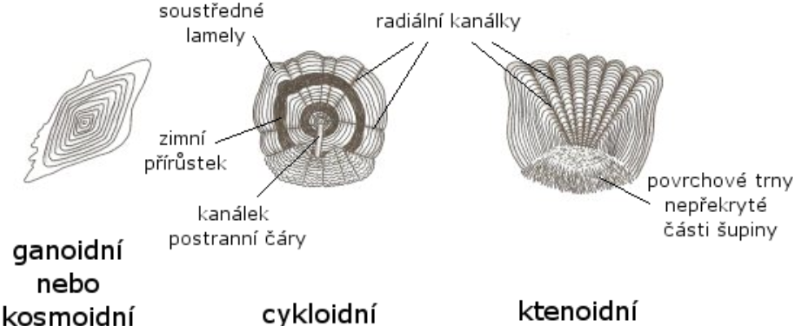
\includegraphics[width=0.49\linewidth]{šupiny}
  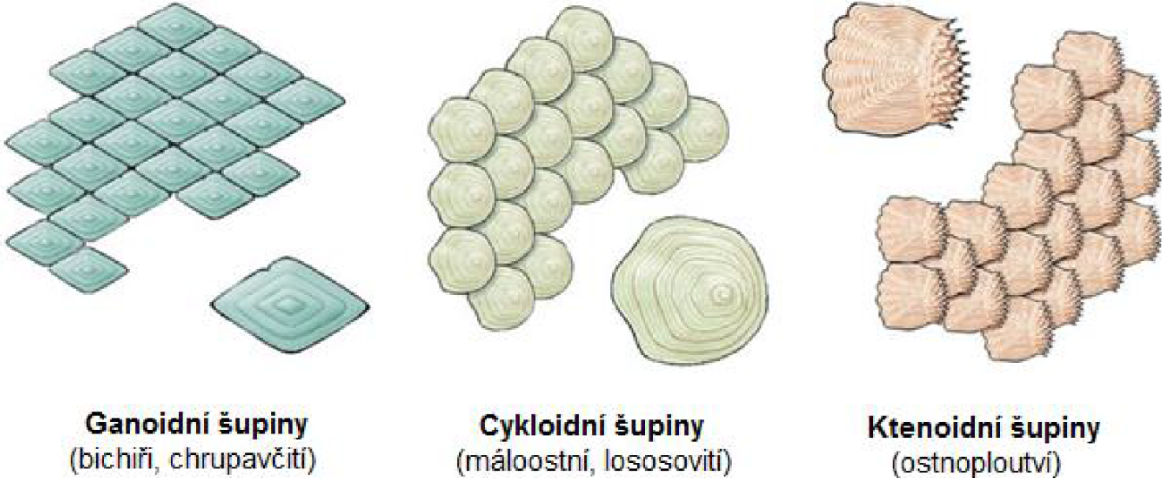
\includegraphics[width=0.49\linewidth]{šupiny_dva}
\end{minipage}

\hspace{-0.03185\textwidth}\begin{minipage}{0.535\textwidth}\raggedleft
  \begin{itemize}
    \item na těle ploutve -- prsní, břišní, hřbetní, řitní a ocasní
    \item ocasní ploutev buď:
    \begin{itemize}
      \item homocerkní -- souměrně laločná
      \item heterocerkní -- nesouměrně laločná
      \item difycerkní -- není laločná
    \end{itemize}
  \end{itemize}
\end{minipage}
\hspace{-0.08\textwidth}\noindent\begin{minipage}{0.455\textwidth}
  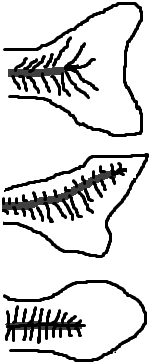
\includegraphics[width=0.09\linewidth]{ocasni_ploutev}
  \hspace{0.1\textwidth}
  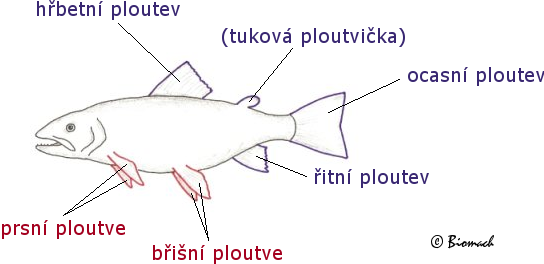
\includegraphics[width=0.75\linewidth]{ploutve}
\end{minipage}

\begin{itemize}
  \item kosti jsou dobře osifikované, osou je páteř (chorda je potlačena obratli)
  \item kosti vznikají osifikací chrupavky
  \item ve svalovině převládá podélný boční sval
  \item mozog, mozog v lebce, 5 částí mozogu
  \item smyslový orgán postranní čára -- rybou proudí voda, jsou zde nervová zakončení -- vnímá proud, teplotu vody, chemoreceptory (čich)
  \item další smysly např. sluch a rovnováha -- vnitřní oko se třemi otolity (balanc šutry, jako u nás), oči bez víček, čočka se neroztahuje a smršťuje, ale posouvá se (podle toho zaostření)
\end{itemize}
\begin{minipage}{\textwidth}
  \begin{itemize}
    \item trávící soustava trubicovitá, hltan, žaludek, střeva, játra, žlučník, slezina, slinivka, zvláštností jsou požerákové zuby -- posouvá potravu hlouběji do úst, ústa buď:
  \end{itemize}
\end{minipage}
\begin{minipage}{0.62\textwidth}\raggedleft
  \begin{itemize}
    \item[]
    \begin{itemize}
      \item svrchní -- ústa směrem nahoru, chytá věci na hladině
      \item koncová -- ústa směrem dopředu, predátoři
      \item spodní -- ústa směrem dolů, vyhrabává živočichy u dna
    \end{itemize}
  \end{itemize}
\end{minipage}
\hfill
\noindent\begin{minipage}{0.38\textwidth}
    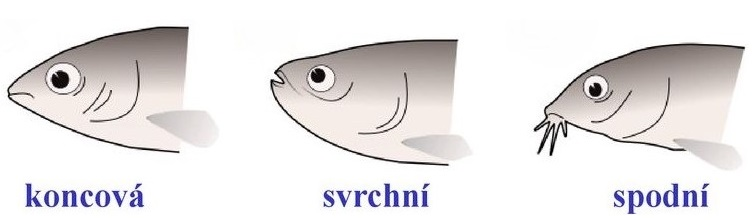
\includegraphics[width=\linewidth]{rybi_huby}
\end{minipage}
\begin{itemize}
  \item venózní (žilné -- neokysl. krev) srdce na břišní straně, červené krvinky jsou velké, oválné a mají jádro
  \item u všech ryb vývod na močopohlavni (urogenitální) bradavce za řitním otvorem
  \begin{itemize}
    \item mořské ryby -- hypoosmotické prostředí -- musí se bránit ztrátám vody, moči je málo, přebytečné soli odstraňují žábrami
    \item sladkovodní ryby -- hyperosmotické prostředí -- nadbytečnou vodu odstraňují močí
  \end{itemize}
  \item většina jsou gonochoristé, zpravidla vejcorodí (97\%), živorodí jsou nepravě živorodí
  \item jikernačka -- samice, jikry -- samiččí pohl. buňky, mlíčňák -- samec, mlíčí -- samčí pohl. buňky, tření -- proces oplození, trdliště -- místo, kde probíhá tření, plůdek -- oplozené vajíčko
  \item péče o potomstvo asi u pětiny druhů (od pouhé úpravy trdliště po péči o potomstvo u koníka mořského)
  \item ryby podle výživy
  \begin{itemize}
    \item všežravé -- všežravé
    \item bentofágní -- u dna, vyhrabávají
    \item planktonofágní -- \uv{filtrátoři}, chytají plankon
    \item dravé -- loví jiné ryby
    \item fytofágní -- \uv{býložravci}
  \end{itemize}
  \item rybí pásma
  \begin{itemize}
    \item pstruhové -- čisté horské potůčky, velký spád, chladná voda, kamenité dno, hodně kyslíku; typicky pstruh, vranka
    \item lipanové -- podhorské potoky a říčky, písčité dno, teplejší, ale čistá voda; kromě lipana hrouzek
    \item parmové pásmo -- střední úseky, široké a hluboké koryto; parma, podoustev, ostroretka
    \item cejnové pásmo -- dolní toky, až stojatá voda; celkově kaprovití
  \end{itemize}
  \item rozdělení v moři
  \begin{itemize}
    \item pelagické -- na volném moři v různých hloubkách do 200 m (sledi, sardinky)
    \item litorální -- v mělčinách při pobřeží
    \item bentické -- obývají mořské dno (platýs)
    \item brakické -- žijící v ústích řek
    \item tažné -- žijí v nějaké vodě, chodí se vytřít do opačné (slaná x sladká)
    \begin{itemize}
      \item katadromní -- za třením z řek do moře (úhoř)
      \item anadromní -- za třením z moře do řek (losos, jeseter)
    \end{itemize}
  \end{itemize}
  \item nadřády Chrupavčití, Mnohokostnatí, Kostnatí
\end{itemize}

\subsubsection{nadřád Chrupavčití}
\begin{itemize}
  \item kostra sekundárně zchrupavčitělá, tvar těla podobný parybám
  \item ekonomicky významní -- kaviár
\end{itemize}

\subsubsection{nadřád Mnohokostnatí}
\begin{itemize}
  \item podlouhlí, dnes skoro vyhynulí
  \item ganoidní šupiny
\end{itemize}

\subsubsection{nadřád Kostnatí}
\begin{itemize}
  \item klasická ryba, charakteristika viz výše
\end{itemize}

\part{infrakmen Čtyřnozí (což je jakoby nad nadtřídou)}%začnu řvát
\begin{itemize}
  \item nemám AAAAAAAAA 6.3.
  \item pleziomorfní a apomorfní znaky vůči rybám
\end{itemize}

\section{třída Obojživelníci}
\begin{itemize}
  \item první jsou to (řád???) krytolebci, mají lebku srostlou s horní čelistí, lebka složená z mnoha kostí (tito jsou předci plazů, savců)
  \item jsou studenokrevní (poikilotermové)
  \item trávicí soustava poměrně krátká (jsou to dravci), většinou nemají zuby, mají dlouhý smotaný jazyk, ukončena kloakou (spol. vyústění trávicí, vylučovací a rozmnožovací sous.)
  \item pátý žeberní oblouk přeměněn v jazylku
  \item kůže oproti rybám podstatně jiná -- je tenká, protože jí dýchají, je hodně prokrvená, ve spodní vrstvě mají chromatofory (pigmentové buňky), kůži svlékají
  \item larvy -- pulci, dýchají vnějšími žábrami, mají vyvinutý proudový orgán
  \item dospělci -- dýchají plicmi a kůží
  \item cévní soustava -- srdce se dvěmi síněmi, jednou komorou, v srdci se okysličená krev mísí s neokysličenou
  \item nervová soustava -- nejvýznamnější částí mozku je střední mozek, ale vyvíjí se už i koncový mozek s polokoulemi, mozeček je malý
  \item u dospělců se vytváří střední ucho s jednou sluchovou kůstkou columellou, mají velké oči se třemi víčky (akomodace pohybem čočky), tzv. parietální oko na temeni (vnímá světlo x tma), vyvinutý čich
  \item dělí se na bezocasé, ocasaté a beznohé
  \item samci a samičky, u ocasatých výrazný pohlavní dimorfismus, u ocasatých vnitřní oplození, v bezocasých vnější
\end{itemize}

\subsection{podtřída Bezocasí (žáby)}
\begin{itemize}
  \item krátké tělo bez ocasu, především souš, dlouhé zadní končetiny
  \item mají zkostnatělou kostru
  \item ledka je kloubně spojena s páteří, což jim dává schopnost otáčet hlavou
  \item žáby mají odlehčenou obličejovou část lebky
  \item žáby mají hrudní kost a nemají žebra (drží ramena)
  \item dlouhatánská pánev, uprostřed urostyl
  \item čtyřprsté přední a pětiprsté zadní končetiny
  \item mládě pulec, má delší střevo (býložravec), prvně zadní končetiny
  \item amplexus -- uchycení při rozmnožování
  \item ropuchy (velké, vodorovná zornice), kuňky (kuňčí reflex -- břicho barevné, vyvaluje ho aby ukázala, že je jedovatá), skokani (kulaté zornice, skokan zelený, hnědý), blatnice (horizontální zornice, velicí pulci), rosničky (rozšířené konce prstů, které fungují jako přísavky, rosnička zelená), pralesničky (šípové žáby)
\end{itemize}

\subsection{podtřída Ocasatí}
\begin{itemize}
  \item nemají hrudní kost, ale mají začátek žeber
  \item protáhlé tělo, více přizpůsobeni vodnímu prostředí
  \item redukovaný sluch, v ústech drobné zuby -- specializovaní predátoři
  \item u mláděte se prvně vyvíjejí přední končetiny
  \item např. mlok (parotida -- jedová žláza u mloka skvrnitého), čolek, axolotl (neotenie -- schopnost rozmnožovat se v larválním stádiu -- v přírodě jsou celý život v larválním stadiu)
\end{itemize}

\subsection{podtřída Beznozí}
\begin{itemize}
  \item nějakej červík, starobylá skupina
\end{itemize}

\section{třída Plazi}
\begin{itemize}
  \item když bereme i s ptáky tak je to monofyletický taxon
  \item blány na vejci (tedy Amniota), bílek a skořápka $\Rightarrow$ můžou definitivně opustit vodní prostředí, blány jsou tři:
  \begin{minipage}{0.8\textwidth}
    \begin{itemize}
      \item amnion -- přímo okolo plodu udržující vodní prostředí
      \item allantois -- blána tvořící vak zajišťující výměnu plynů s okolím a skladování moči
      \item serosa -- blána okolo celého žloutku (plod, žloutek, allantois)
    \end{itemize}
  \end{minipage}
  \hfill
  \noindent\begin{minipage}{0.2\textwidth}
      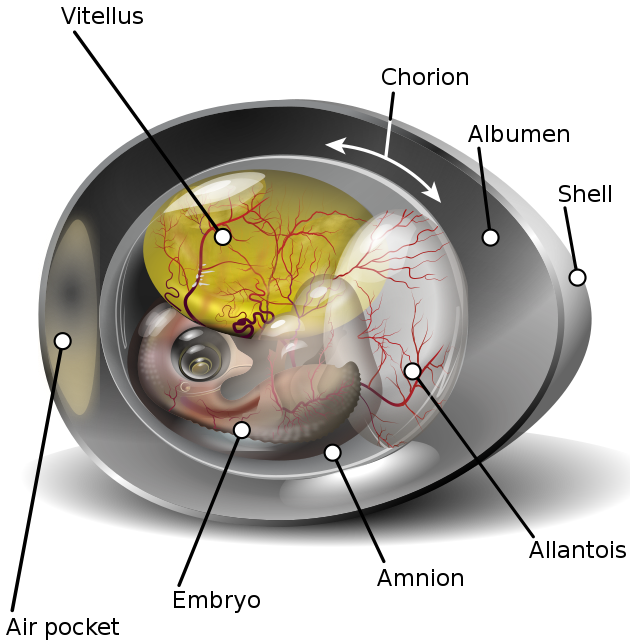
\includegraphics[width=\linewidth]{blany}
  \end{minipage}
  \item všichni dýchají plícemi, nemají larvální stádia
  \item plně osifikovaná kostra, pohyblivé spojení (atlas, axis) lebky s páteří, vznik krku (krční páteře), mají hrudní koš (žebra, hrudní kost), ten svírá plíce, takže potřebují koš roztahovat $\Rightarrow$ většina (kromě želev) mají nově mezižeberní svaly
  \item oproti obojživelníkům pokožka suchá (chybí žlázy), krytá šupinami (kontinuálně z kůže, nejdou oddělit jako u ryb), můžou se objevovat chromatofory (barvoměna, např. chameleoni)
  \item přešli na souš protože tam neměli konkurenci (nebyli tam dravci) a byl tam dostatek zdrojů (už tam jsou rostliny a bezobratlí)
  \item protože jsou na souši tak musí minimalizovat vylučování vody -- moč je zahuštěná a kašovitá, místo močoviny vylučují kyselinu dusičnou
  \item mají končetiny, a to kráčivé, jsou mohutné protože musí udržet váhu těla (chodím po nich, nemám vztlak vody), nejsou pod tělem -- jsou podél těla, končetiny přichyceny pohyblivě a už ne na lebku, v končetinách se jim již vyvíjí postavení kostí podobné našim
  \begin{itemize}
    \item os humerus -- u nás kost pažní (rameno -- loket)
    \item os ulna -- kost loketní (loket -- malík)
    \item os radius -- kost vřetenní (loket -- palec)
    \item tarsus -- kosti zápěstní (uchycení na zápěstí)
    \item metatarsus -- kosti záprstní (uchycení na prsty)
  \end{itemize}
  \item mají dokonalejší plíce (už nemůžou dýchat pokožkou), dokonalejší oběhová soustava a srdce -- už mají dva oběhy (malý plicní, velký tělní) a srdce má dvě síně a dvě komory, ale komory jen částečně přehrazené takže stále dochází k částečnému míchání okysličené a odkysličené krve (plně oddělené až u krokodýlů)
\end{itemize}

\end{document}
